%%%%%%%% ICML 2018 EXAMPLE LATEX SUBMISSION FILE %%%%%%%%%%%%%%%%%

\documentclass{article}

% Recommended, but optional, packages for figures and better typesetting:
\usepackage{microtype}
\usepackage{graphicx}
\usepackage{subfigure}
\usepackage{booktabs} % for professional tables
\usepackage{amsmath, amssymb}

\usepackage[utf8]{inputenc}
\usepackage[T1]{fontenc}
\usepackage{hyperref}
\usepackage{url}
\usepackage{booktabs}
\usepackage{amsfonts}
\usepackage{nicefrac}
\usepackage{microtype}
\usepackage{xcolor}
\usepackage{lipsum}
% \usepackage[nomarkers,nolists,figuresonly]{endfloat} %comment out when finish
\usepackage{booktabs}
\usepackage{multirow}
\usepackage{float}
\usepackage{subcaption}


% hyperref makes hyperlinks in the resulting PDF.
% If your build breaks (sometimes temporarily if a hyperlink spans a page)
% please comment out the following usepackage line and replace
% \usepackage{icml2018} with \usepackage[nohyperref]{icml2018} above.
\usepackage{hyperref}

% Attempt to make hyperref and algorithmic work together better:
\newcommand{\theHalgorithm}{\arabic{algorithm}}

% Use the following line for the initial blind version submitted for review:
\usepackage[accepted]{icml2018}

% If accepted, instead use the following line for the camera-ready submission:
%\usepackage[accepted]{icml2018}

% The \icmltitle you define below is probably too long as a header.
% Therefore, a short form for the running title is supplied here:
\icmltitlerunning{CS234: Reinforcement Learning Winter 2025 - Final Project}

\begin{document}

%%%%%%%%%%%%%%%%%%%%%%%%%%%%%%%%%%%%%%%%%%%%%%%%%%%%%%%%%%%%%%%%
%%%%%%%%%%%          HEADER SECTIONS HERE            %%%%%%%%%%%
%%%%%%%%%%%%%%%%%%%%%%%%%%%%%%%%%%%%%%%%%%%%%%%%%%%%%%%%%%%%%%%%


\twocolumn[
\icmltitle{Enhancing Game Control Through \\
Hybrid Reinforcement Learning
}

\begin{icmlauthorlist}
\icmlauthor{Danhua Yan}{to}
\end{icmlauthorlist}

\icmlaffiliation{to}{Department of Computer Science, Stanford University}
\icmlcorrespondingauthor{Danhua Yan}{dhyan@stanford.edu}

% You may provide any keywords that you
% find helpful for describing your paper; these are used to populate
% the "keywords" metadata in the PDF but will not be shown in the document
% \icmlkeywords{Machine Learning, ICML}

\vskip 0.3in
]

% this must go after the closing bracket ] following \twocolumn[ ...

% This command actually creates the footnote in the first column
% listing the affiliations and the copyright notice.
% The command takes one argument, which is text to display at the start of the footnote.
% The \icmlEqualContribution command is standard text for equal contribution.
% Remove it (just {}) if you do not need this facility.

%\printAffiliationsAndNotice{}  % leave blank if no need to mention equal contribution
% \printAffiliationsAndNotice{\icmlEqualContribution} % otherwise use the standard text.
\printAffiliationsAndNotice{} % otherwise use the standard text.



%%%%%%%%%%%%%%%%%%%%%%%%%%%%%%%%%%%%%%%%%%%%%%%%%%%%%%%%%%%%%%%%
%%%%%%%%%%%           MAIN SECTIONS HERE             %%%%%%%%%%%
%%%%%%%%%%%%%%%%%%%%%%%%%%%%%%%%%%%%%%%%%%%%%%%%%%%%%%%%%%%%%%%%


\begin{abstract}
This document provides a basic paper template and submission guidelines.
Abstracts must be a single paragraph, ideally between 4--6 sentences long.
Gross violations will trigger corrections at the camera-ready phase.
\end{abstract}

\section{Introduction}

% What is the problem that you will be investigating ? Why is it interesting ?
% What literature have you already surveyed or will be 
% examining to provide context and background ?

Training Reinforcement Learning (RL) agents usually requires a substantial 
amount of data and exploration to find an optimal policy. In many complex 
games, the challenges of high-dimensional state spaces, sparse rewards, and 
complex dynamics make training agents using pure exploration particularly 
inefficient. Moreover, in cases where exploration opportunities are limited or 
costly, the RL agent might fail to learn any usable policies \cite{Coletti2023EffectivenessOW}. 
Such inefficiency not only slows down learning but also increases the risk of 
converging to policies that are far from optimal.

The research field of bootstrapping an RL agent's policy from demonstrations or 
imitation learning shows significant promise. Various hybrid paradigms that 
combine human guidance as offline RL and agent exploration as online RL have 
shown they can accelerate policy learning and achieve above-demonstration 
performance \cite{hester_dqfd_2017,nair_bcrl_overcoming_2018, song_hybrid_2023, 
ren_hybrid_2024, Coletti2023EffectivenessOW}.

This project investigates how hybrid RL (HRL) can effectively enhance game control 
through guided explorations of the agent. It aims to evaluate the potential for 
achieving performance that surpasses the demonstration level.

\section{Related Work}

\clearpage

\section{Data and Environement}
In this project, we leverage the \texttt{stable-retro} library to create an OpenAI Gym 
environment for training an agent to play the NES game Super Mario Bros, level 1-1. The 
default integration of the environment encapsulates the game into the in-game visual 
frame as a matrix $I \in \mathbb{R}^{H \times W \times 3}$, where each element takes an 
integer value between 0 and 255, representing the RGB channels of the frame. The action 
of pressing 9 buttons on NES controllers is represented as a vector 
$\mathbf{a} = (a_1, a_2, \dots, a_9) \in \{0, 1\}^9$, where each button can be toggled 
independently, resulting in a total of 512 discrete action spaces. The default reward 
is the change in the $x$-axis position $\Delta x$ moved by Mario. In-game metadata, including 
scores, time left, and positions of Mario, can also be retrieved for each timestep $t$.

\subsection{Human Demonstration Data}
\label{sec:hd_data}
To record human demonstrations, we implemented scripts to save gameplay 
interactions with the environment via a game controller. 
We recorded five gameplays by amateur players $\{\tau_{\text{HD}}^{i}\}_{i=1}^{5}$, 
each successfully completing Level 1-1 without losing a life.
Each episode $i$ is 
saved as $\tau_{\text{HD}}^{i} = \{(s_t, a_t, r_t, d_t, m_t)\}_{t=0}^{T}$, where each 
element represents the observation, action, reward, termination boolean, and 
metadata.  
Additionally, a single trajectory 
of game emulator states is saved every 50 steps, 
$\tau_{\text{ES}} = \{ s_t \mid t \in \{ 50k \mid k\in \mathbb{N}, 50k \leq T \} \}$,
used for resetting RL agents 
to start from a state along the human demonstrated trajectory.

\subsection{Customized Game Environement}

To frame the game as a solvable RL problem within a reasonable time, we made 
the following custom modifications to the default game integration:

\textbf{Action Space} 
The default 512 discrete action space includes all possible joystick button 
combinations, most of which are not meaningful for controlling Mario. We 
reduced the action space to 3 commonly used button combinations (see 
Appendix \ref{a1:custom_env}).

\textbf{Termination States}
The default game termination occurs when Mario exhausts all lives or the 400 
second time limit for Level 1-1 is reached. We employ stricter termination 
conditions: 1) Mario has only one life, and the game terminates immediately if 
he loses it; 2) If Mario remains stuck at the same position without moving 
right for 10 seconds, the game is terminated.

\textbf{Reward Function}
The game's scoring system provides sparse rewards for defeating enemies, 
collecting coins or power-ups, and successfully completing the level.
We modify the reward function to provide dense rewards, incorporating scores, 
encouraging rightward movement with milestones, and penalizing time consumption 
and termination without success:

\begin{align*}
      \mathcal{R} = &\Delta s + \beta_x \Delta x + \beta_t \Delta t + \mathbf{1}[d_{\text{milestones}} = 1] M\\
      & + \mathbf{1}[d_{\text{timeout}} = 1] T_t + \mathbf{1}[d_{\text{death}} = 1] T_d
\end{align*}

where $\Delta s$ is the score earned since the last state, $\Delta x$ is the 
movement, $\Delta t$ is the time spent, $\beta$ are coefficients, $M$ is the 
milestone score at 10\%, 20\%, etc., of the level, and $T_t$ and $T_d$ are 
penalties for timeout and death terminations.

\textbf{Sampling Rate}
To ensure smooth rendering, the game runs at 60 fps. However, consecutive 
frames exhibit minimal differences. Following \cite{feng2024mario}, 
we reduced the sampling rate to 15 fps to enhance efficiency.


\section{Approach}
In this section, we describe baseline and three different hybrid reinforcement 
learning approaches in controlling Mario for completing level 1-1.

\subsection{Policy Training Architectures}

\begin{figure}[htbp]
      \centering
      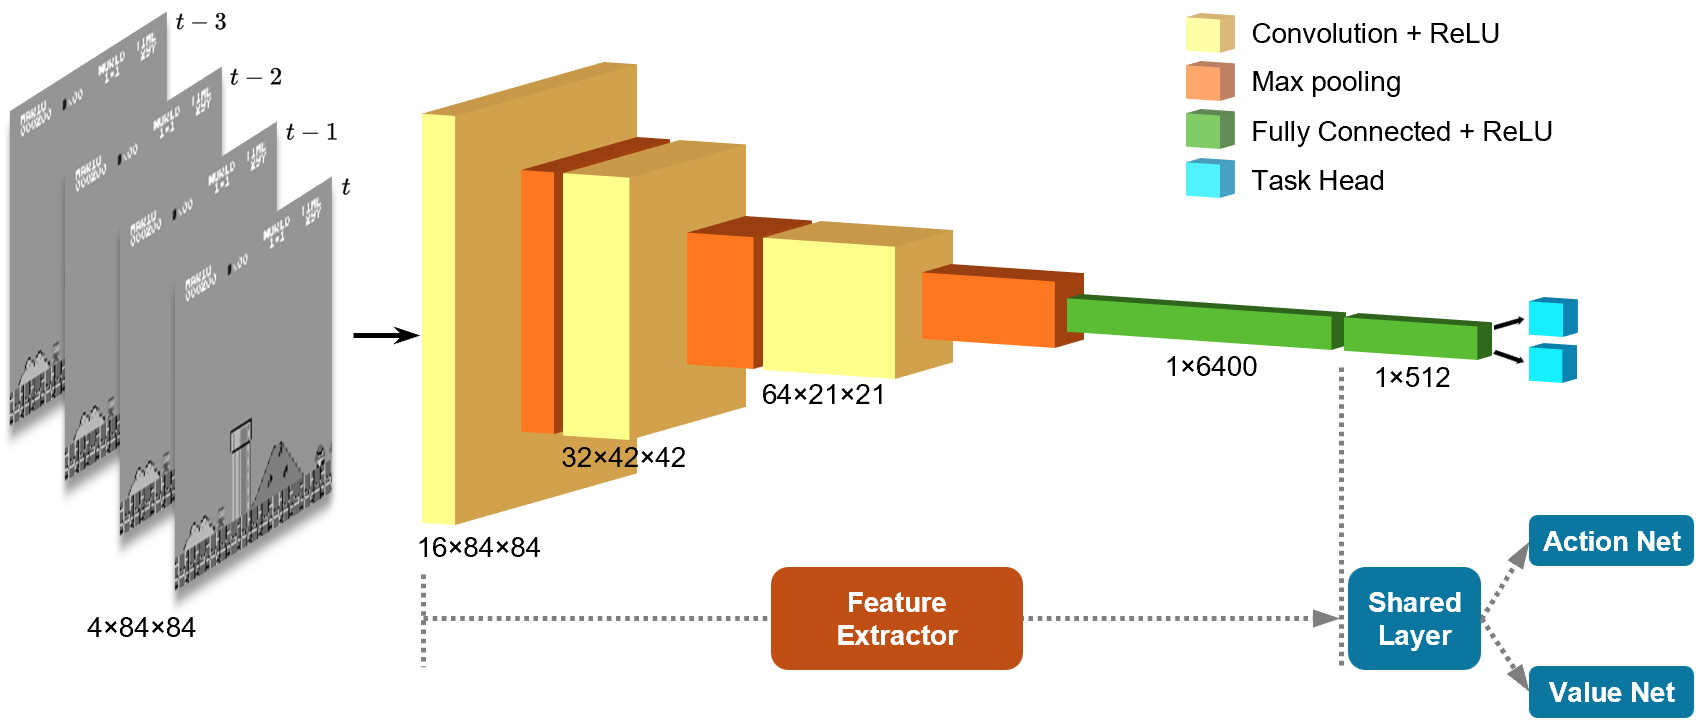
\includegraphics[width=\columnwidth]{figures/architecture.png}
      \caption{PPO agent architecture for playing Super Mario Bros.
      Four downsampled gameplay frames are stacked 
      to represent the current state $s_t$, as input to the CNN actor-critic PPO
      networks.}
      \label{fig:arch}
\end{figure}

\textbf{State Representation}
Due to the presence of moving enemies (\textit{e.g.}, Goombas, Koopa Troopas) 
and power-ups, \textit{Super Mario Bros.} exhibits non-Markovian dynamics.
As a result, incorporating temporal structure in the state representation is 
crucial for accurately estimating enemy movements and other dynamic changes. 
To capture these temporal dependencies, we define the state $s_t$ at time $t$ 
as a stack of four consecutive gameplay frames, $\{ f_{t-3}, \dots, f_t \}$, 
preserving local temporal dynamics (see Figure \ref{fig:arch}). 
Each frame is downsampled from its original RGB representation to a 
single-channel grayscale image and resized to $84 \times 84$ pixels.

\textbf{Network Architectures}
All baselines and HRL approaches use the same architecture 
(Figure \ref{fig:arch}). The feature extractor is a CNN 
$\phi_s = \mathcal{F}(s;\phi)$ that maps the stacked state 
representation \(4 \times 84 \times 84\) to a dense feature 
representation. The CNN has three convolutional layers with 16, 32, 
and 64 channels, respectively. Each convolution uses a \(3 \times 3\) 
kernel with stride 1 and padding 1, followed by ReLU activation and 
\(2 \times 2\) max pooling, halving the spatial dimensions. 
The PPO actor-critic policy 
is a multi-head MLP network $a, V = \mathcal{M}(\phi_s; \theta)$ with a 
shared fully connected hidden layer of 512 units and 
ReLU activation, and two linear heads:
the action net $a \sim \pi_\theta(s|a) = M_a(\phi_s;\theta_a)$,
and the value net ${\hat V} = M_V(\phi_s;\theta_V)$.
For BC, it matches the PPO with just action net:
$a \sim \pi_{\text{BC}}(s|a) =
\mathcal{M}_{\text{BC}}(\mathcal{F}(s;\phi_{\text{BC}});\theta_{\text{BC}})$.


\subsection{Baselines}
Here we shall establish performance of offline-only and online-only RL approaches
as baselines to compare against future HRL approaches and human demonstration trajectories. 

\subsubsection{Behavior Cloning (BC)} 
BC is an offline approach using supervised 
learning to map state-action pairs from human demonstrations. We learned 
a BC policy $\pi_{\text{BC}}(s|a) =
\mathcal{M}_{\text{BC}}(\mathcal{F}(s;\phi_{\text{BC}});\theta_{\text{BC}})$
using $(s,a)$ pairs from human demonstration data $\tau_{\text{HD}}$ as mentioned
in section \ref{sec:hd_data}.

\subsubsection{Proximal Policy Optimization (PPO)} 
PPO serves as an online baseline. We extended the 
\texttt{stable-baseline3} PPO implementation, utilizing the 
CNN feature extractor $\mathcal{F}(s;\phi)$ and the two-head 
MLP policy network $a, V = \mathcal{M}(\phi_s; \theta)$. 
Parameters $\phi$ and $\theta$ are updated via gradient 
descent per rollout iteration.
Here we denote the policy learned by PPO as 
$\pi_\theta(s|a) = M_a(\mathcal{F}(s;\phi);\theta_a)$.


\subsection{Hybrid Reinforcement Learning (HRL)}
We explore three HRL paradigms, leveraging pre-trained BC policies or 
directly using human demonstration data in PPO policy learning.

\subsubsection{BC-Initialized PPO}
This approach initializes PPO explorations using pre-trained behavior 
cloning weights. These weights provide a biased prior for state and 
action distributions, giving the agent a reasonable initial policy 
for exploration. 
Instead of initializing the model with random parameters 
$\phi_0$ and $\theta_0$, i.e., $a, V = \mathcal{M}_0(\mathcal{F}_0(s;\phi_0); 
\theta_0)$, we warm-start the feature extractor $\phi_0 \leftarrow 
\phi_{\text{BC}}$ and/or the policy network $\theta_0 \leftarrow 
\theta_{\text{BC}}$ in this approach.

\subsubsection{BC-Constrained PPO}
This approach constrains the PPO policy to remain close to the pre-trained BC 
policy by adding a KL-divergence term to the loss function:

\begin{align*}
      \mathcal{L}(\theta) 
      &= \mathcal{L}_{\text{PPO}}(\theta) +
      \lambda \mathbb{E}_{s \sim \mathcal{D}} \bigg[ \sum_{a} \pi_{\theta}(a | s) \log 
      \frac{\pi_{\theta}(a | s)}{\pi_{\text{BC}, \theta_{\text{BC}}}(a | s)} \bigg],
\end{align*}
where $\mathcal{L}_{\text{PPO}}$ is the default PPO loss, $\lambda$ is the hyperparameter
controlling the strength of the divergence loss.

\subsubsection{Assisted Explorations}
This approach aims to shape the exploration process using human trajectories. 
The key idea is to reset the rollout to progressively more challenging starting 
points for the agent, encouraging the learning process \cite{florensa2018reversecurriculumgenerationreinforcement}. 
\cite{salimans2018learningmontezumasrevengesingle} proposed reversing the human 
gameplay trajectory as resets to effectively encourage learning. Inspired by 
their approach, we propose a simpler version of resets using an exponential 
decay schedule, instead of running indefinitely until each reset reaches a 
certain performance threshold.

The exponential decay schedule for PPO resets works as follows: given a target 
training iteration count $N$ and $k$ resets along the trajectory, we want the 
$i$-th state to be reset for rollout $f(i)$ times, such that $f(i)$ follows a 
discrete exponential distribution $f(i) \sim r^i$, and $\sum_{i=1}^{k} f(i) 
\approx N$. Here, $r$ is the decay factor, where $0 < r < 1$, that smaller $r$ decays 
faster. The PPO rollouts start from the $k$-th human state from 
$\tau_{\text{ES}}$ (see section \ref{sec:hd_data}) $f(k)$ times, then move to 
the $(k-1)$-th state $f(k-1)$ times, and so on, until exhausting all states in 
$\tau_{\text{ES}}$. If there are still training steps remaining, the rollouts 
start from the initial state $s_0$.

The intuition behind this approach is to distribute resets strategically 
within a given training iteration count. States closer to the winning 
state (later states) are easier and thus get less practice than the 
earlier, more difficult states. This schedule effectively distributes 
learning along good state trajectories within limited training time, 
aiding efficient explorations.




\section{Experiments}
In this section, we present experimental results for the aforementioned 
approaches. All experiments are trained on a single Nvidia GeForce RTX 4070 Ti 
SUPER 16GB GPU.

\subsection{Baselines}
All $(s_t, a_t)$ 
pairs are split into \texttt{train} and \texttt{dev} sets in a 7:3 ratio. 
With a batch size of 32 and cross-entropy loss, the full network 
$\pi(\mathcal{F}(s; \phi);\theta)$ is trained for 500 epochs using 
AdamW optimizer with a learning rate of $10^{-4}$. Early termination 
occurs after 50 epochs based on \texttt{dev} data accuracy.

In each iteration, the agent will rollout for 512 steps,
update the networks for 10 epochs with batch size 32, for a total 200 iterations.
Here we use hyperparameters of learning rate
$3\times10^{-5}$, clip range of 0.02, and entropy loss
coefficient of 0.01.

\begin{figure}[htbp]
      \centering
      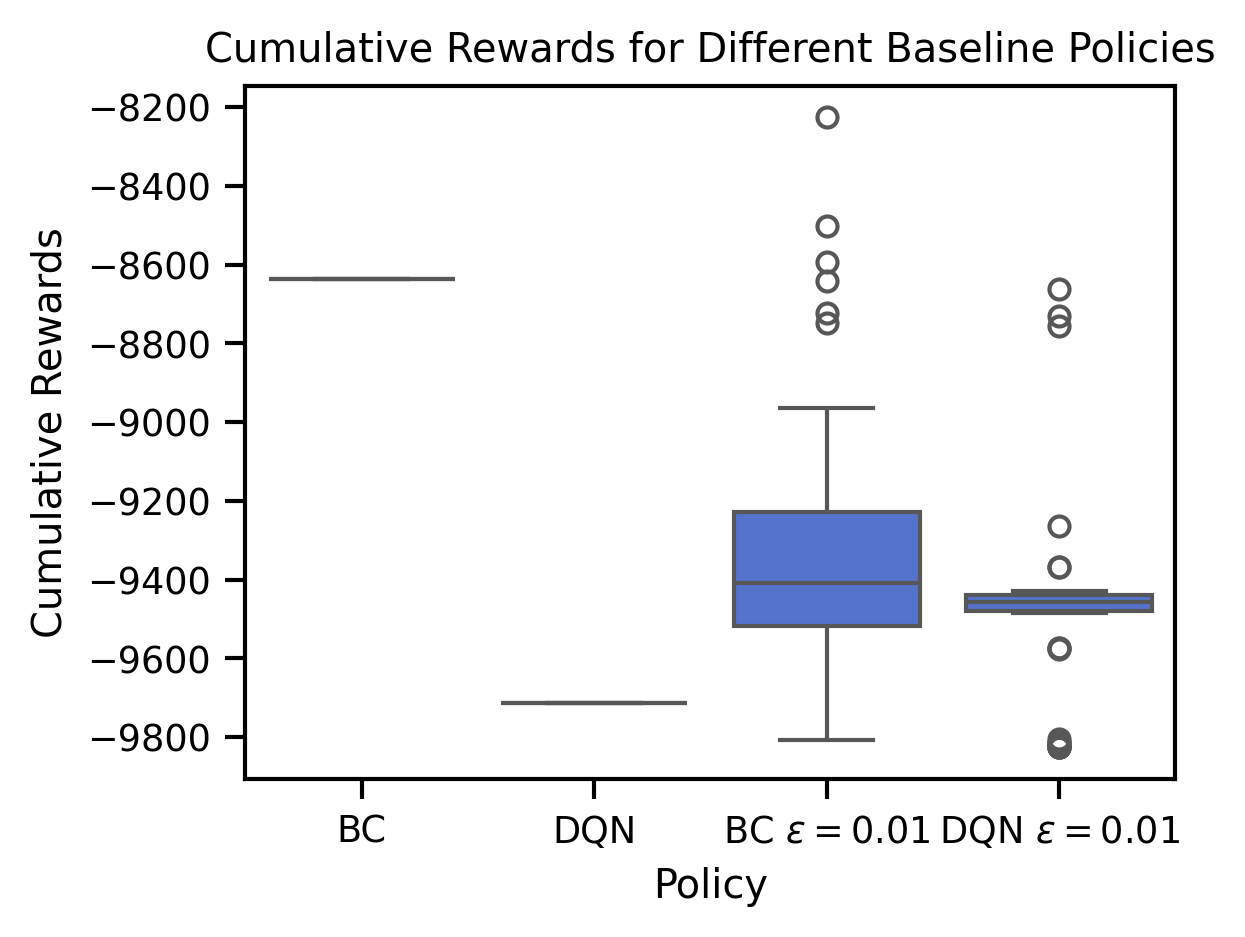
\includegraphics[width=0.8\columnwidth]{figures/cum_rewards_baseline.png}
      \vspace{0.5cm} % adjust vertical space as needed
      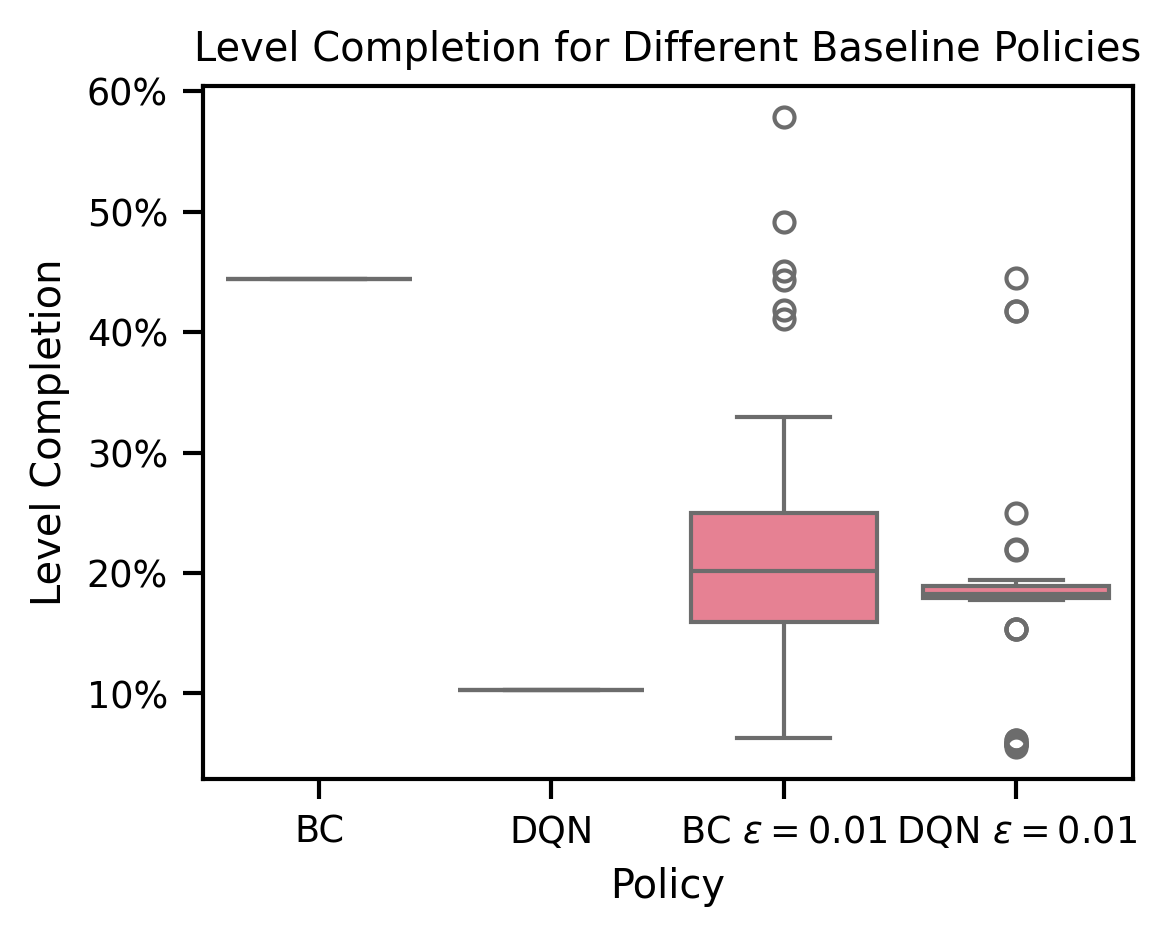
\includegraphics[width=0.8\columnwidth]{figures/completions_baseline.png}
      \caption{Baseline policies in-game performance statistics for 50 episodes each.}
      \label{fig:baseline_policies}
\end{figure}

DQN policy $\pi_{\text{DQN}}$ and BC policy $\pi_{\text{BC}}$ are learned 
through the aforementioned setups. It took about 8 hours to train 
$\pi_{\text{DQN}}$ and 1 hour for $\pi_{\text{BC}}$ on the GPU. After training, 
we rolled out 50 game plays for each policy to evaluate their performance based 
on cumulative rewards at terminated states and game completion percentage, 
defined as the total x-scrolling distance compared to the end of the level. 

Since the trained policies are deterministic, we introduce some stochasticity 
by adding a small $\epsilon=0.01$ where the policy will act randomly. This evaluates 
the robustness under perturbations, especially in complex game settings where 
encountering enemies and obtaining power-ups can significantly change the best 
actions to take. For all gameplays, the initial action is set to move right 
regardless of the policies to avoid Mario being stalled.

Both policies failed to complete the game level successfully.
$\pi_{\text{BC}}$ demonstrates significantly better performance in terms of 
cumulative rewards and game completions under the deterministic setup, despite 
taking only 1/8 of the time to train compared to $\pi_{\text{DQN}}$ and using 
only 5 human-demonstrated trajectories, as shown in Figure 
\ref{fig:baseline_policies}. However, $\pi_{\text{BC}}$ suffers from greater 
performance degradation when random perturbations are introduced. It exhibits 
higher variance in performance in stochastic setups.
$\pi_{\text{DQN}}$, on the other hand, is rather difficult to train. In the 
complex game environment, though rewards are not sparse, encountering enemies 
and power-ups makes the Markov assumptions less valid, and the pipes in the 
game create challenges for the agent to explore states effectively. Thus, the 
explorations are rarely sufficient to learn good $Q$ value estimations even 
after 2500 episodes (see Appendix \ref{a2:dqn}). The trained $\pi_{\text{DQN}}$ 
does not compare with $\pi_{\text{BC}}$ in deterministic settings but shows 
superior stability in terms of variance when randomness is introduced, with 
increased performance when acting stochastically. This illustrates that the 
current exploration is sub-optimal, and when exploring guided by human 
demonstrations, it could surpass $\pi_{\text{BC}}$ in performance.

\section{Next Steps}
Above initial results show the expected performance of baselines. The remaining 
work of the project involves finishing the implementation of the HRL algorithms 
and evaluating the performance of each approach.

\subsection{Deep \textit{Q}-Learning from Demonstrations (DQfD)}

Following the DQfD (Deep \textit{Q}-Learning from Demonstrations) framework by 
\cite{hester_dqfd_2017}, we incorporate human demonstrations into the replay 
buffer $\mathcal{D}$ of DQN to control explorations. This builds on the already 
implemented DQN framework, where the loss functions and replay buffer 
trajectories are modified to include human demonstrations.

\subsection{PPO with Behavior Cloning Warm-start}

Inspired by \cite{Coletti2023EffectivenessOW}, this approach leverages 
$\pi_{\text{BC}}$ trained model weights as a warm-start, then further leverages 
PPO for policy fine-tuning. PPO's property of 
prohibiting significant updates to the policies ensures that explorations will 
be around human demonstrations, with the possibility to improve and surpass 
human performance.

\subsection{Evaluations}
We will evaluate the approaches using both quantitative and qualitative metrics. 
Quantitatively, performance will be measured via cumulative reward, level 
completion rate, and distance traversed per episode, plotted as learning curves 
against training episodes or timesteps. Multiple independent runs will ensure 
statistical significance. Sample efficiency will be analyzed by measuring 
interactions required to reach performance thresholds and wall-clock training 
time. Qualitatively, gameplay visualizations and trajectory overlays will 
provide insights into behavioral strategies.


\bibliography{ref}
\bibliographystyle{icml2018}

\clearpage
\appendix
\renewcommand{\thefigure}{A\arabic{figure}}
\renewcommand{\thetable}{A\arabic{table}}
\setcounter{figure}{0}
\setcounter{table}{0}
\onecolumn
\section{Appendix}
\subsection{Custom Environment}
\label{a1:custom_env}

The default 512 discrete action space captures all possible joystick button 
combinations. However, most of these combinations are not meaningful for 
controlling Mario. From the human demonstration trajectories, we narrowed down 
the action space to 3 common used button combinations.
Then the action vector is labeled as integers (0-9, following below orders)
as discrete action space for the environment.

\begin{verbatim}
# List of meaningful button combinations used in gameplay
meaningful_actions = [
      [0, 0, 0, 0, 0, 0, 0, 0, 0],  # No action
      [0, 0, 0, 0, 0, 0, 0, 1, 0],  # Right
      [0, 0, 0, 0, 0, 0, 0, 1, 1],  # Right + A (Jump)
]
\end{verbatim}

\subsection{DQN Training}
\label{a2:dqn}

$\pi_{\text{DQN}}$ is rather difficult to train. In the 
complex Super Mario Bros game environment, though rewards are not sparse, encountering enemies 
and power-ups makes the Markov assumptions less valid, and the pipes in the 
game create challenges for the agent to explore states effectively.

As seen in Figure \ref{figa:dqn}, the loss has increased as random explorations 
reduced. The rewards grow very slowly and drastically drop at the end. We 
observed the policy was stuck in a reward-hacking phase where Mario moves only 
to the left until time-out termination. This reduces the risks of getting stuck 
at further pipes with lower rewards and encountering enemies. Such behaviors 
might be addressed by tuning reward functions and exploring if HRL can help 
with this situation.

\begin{figure}[htbp]
\centering
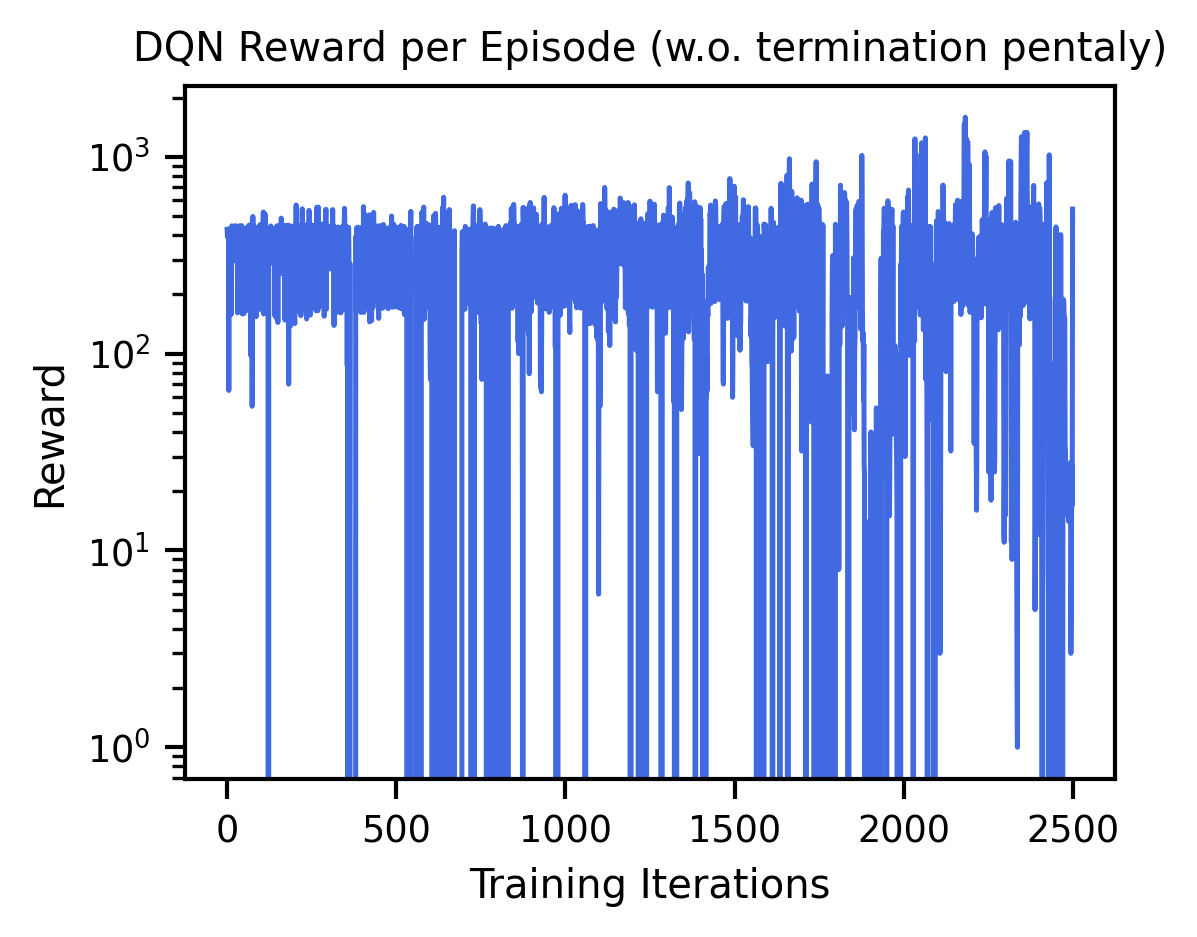
\includegraphics[width=0.45\columnwidth]{figures/dqn_rewards.png}
\hspace{0.5cm} % adjust horizontal space as needed
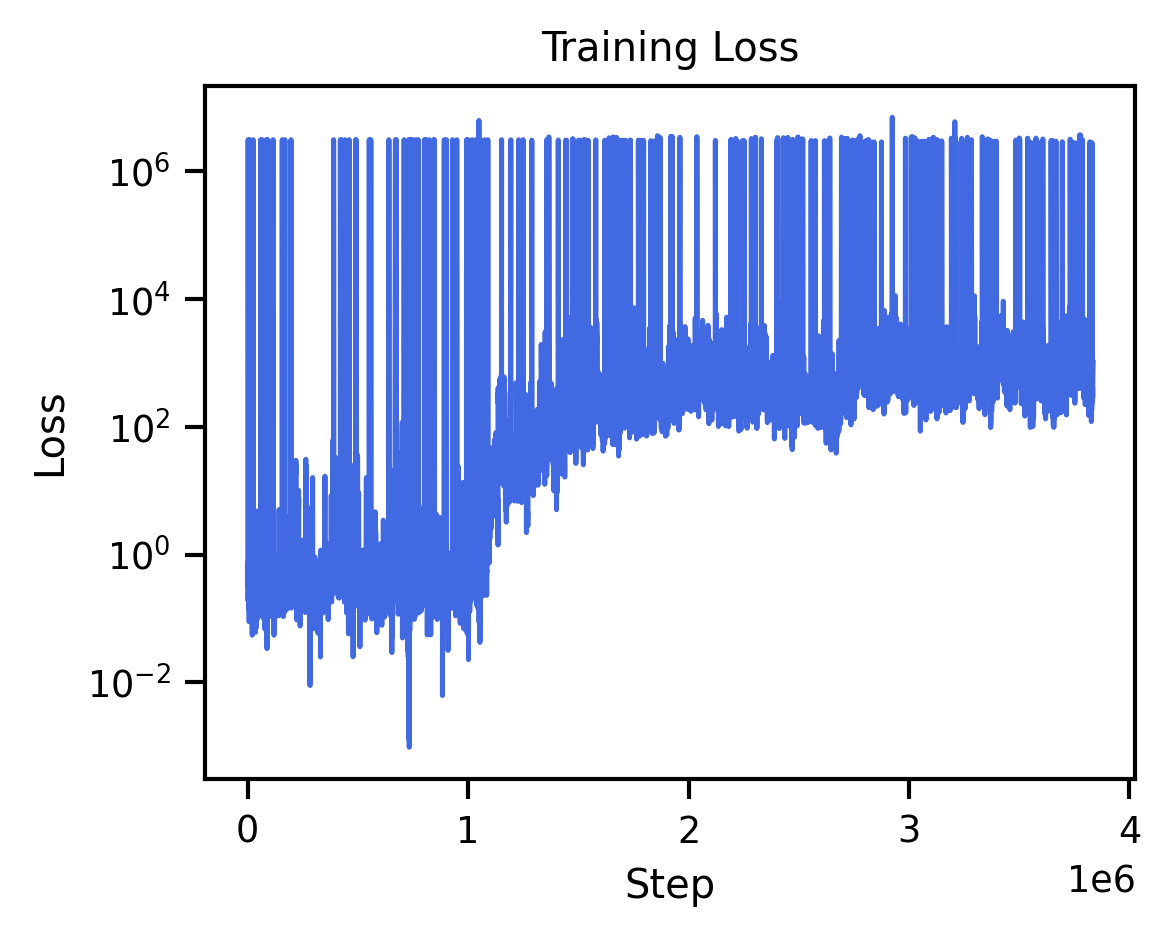
\includegraphics[width=0.45\columnwidth]{figures/dqn_loss.png}
\caption{DQN training loss and rewards}
\label{figa:dqn}
\end{figure}



\end{document}